\section{Background}
\label{background}

This section briefly reviews essential background on vehicular security and message authentication codes. 
The experienced reader may wish to skip to Section~\ref{problem}. 
We assume the reader is familiar with cryptographic hash functions as explained, for example, by Stinson~\cite{Sti} and NIST~\cite{FIPS-180-4}.
\textcolor{red}{Note: You mentioned Stinson on the last draft notes -- this is the book Cryptography - Theory and Practice?---YES}.

\subsection{ECUs}
The Electronic Control Units (ECUs) found in an automotive computer network are low-power, single-purpose devices. ECUs on the CAN bus control many components in a modern automobile, from headlights and window controls, to brakes and engine. They are not typically designed with security in mind and frequently comprise a basic CAN bus transceiver, basic message processor, and an actuator. The message processor identifies whether or not a message being broadcast is interesting to the ECU and arbitrates bus rights with the other ECUs. 

\subsection{The CAN Bus}
The CAN bus is a simple, low-speed bus designed to network simple nodes. In an automotive environment, 
it typically runs at 500~kbps.\footnote{kilobits per second (kbs).} As shown in Figure~\ref{fig-frame}, 
a message contains an 11-bit identifier field and 
a data payload, as well as some control bits. Figure~\ref{fig-frame} shows the data payload as 8~bits, but
it is typically 8 to 64~bits [ref?].
The payload of up to 8~bytes is the most important element, as any MAC must fit into this frame or use a more complex multi-frame data transmission protocol that may or may not be supported on all ECUs. 

Ideally, and in the case of Mini-MAC, the MAC can fit into the payload with the data, thus not increasing bus utilization. Data captured by the authors from a 2010 Toyota Prius show that a large percent (61\%) of messages use no more than four bytes of data in the payload.

% On the diagram, there are 55 bits including 8 data bits. In practice, the 8 bit field is 64 bits, 
% so the total packet is 111 bits. So there are more than 64 total bits sent, but not more than 64 data bits.

	\begin{figure*}
		\centering
		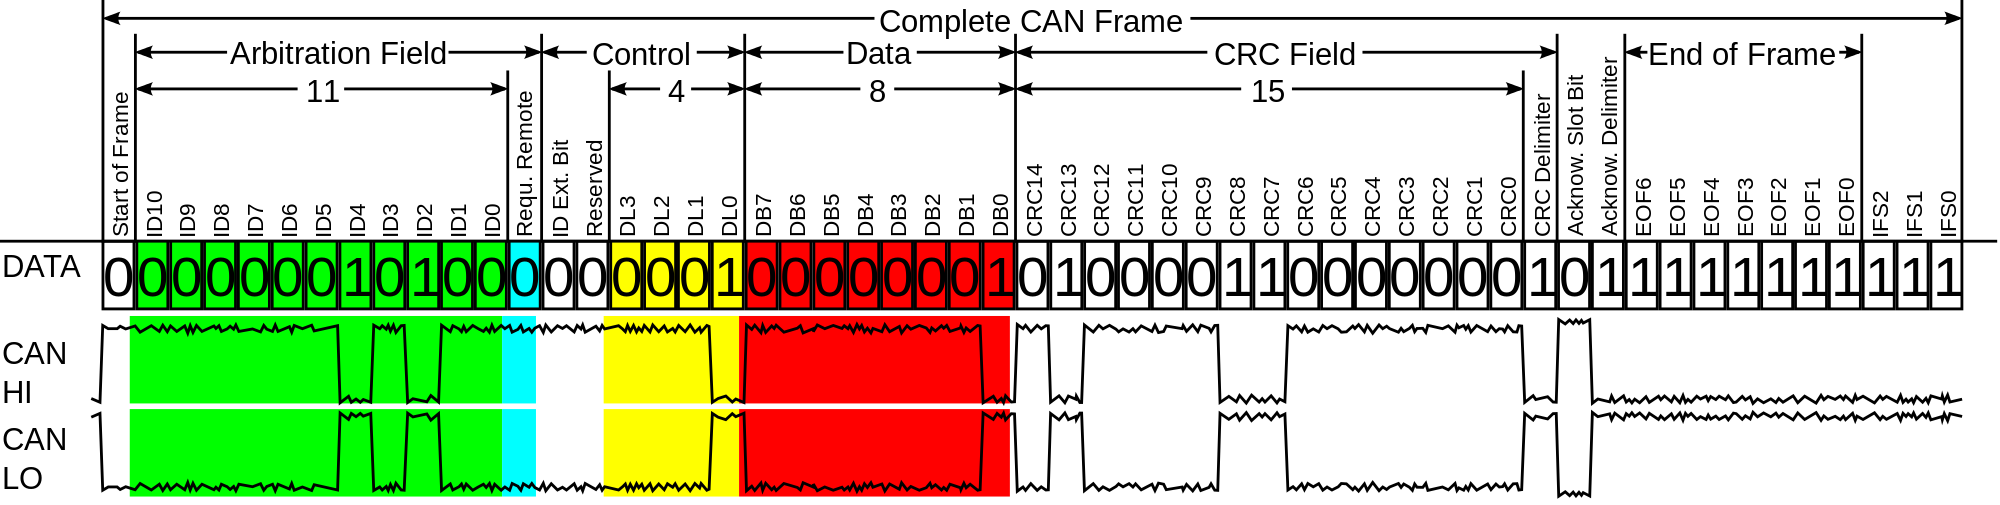
\includegraphics[width=\linewidth]{figures/can_frame.png}
		\caption{The CAN frame~\cite{} [need to cite fig].  
		Each message on the CAN bus is a structured sequence of 55--111~bits including 8--64 data~bits.}
		\label{fig-frame}
	\end{figure*}

\subsection{Bus Access}

To spoof or replay messages on the CAN bus, the attacker must have access to it.
There are several ways to access the CAN bus:  (1) There is a
physical connection through the On-Board Diagnostic (OBD-II) port, 
typically located underneath the steering wheel.  An attacker might hide
access to this port by splicing into unexposed wires.
(2) An attacker might corrupt an ECU by rewriting its firmware. An attacker might
do so while the car is being serviced or by entering the car while it is parked.
(3) An attacker might gain access to the CAN bus by exploiting or corrupting a peripheral
device connected to it, such as a cellular phone, audio system, or Bluetooth
radio.  For example, Checkowa~\cite{Checkoway-2011} gained bus access by packing 
malware into a WMA audio file played on the car stereo. [give another example
of wireless access from drive-by attacker]

Despite many demonstrated security flaws, automotive 
manufacturers have been unreasomnably hesitant to acknowledge the vulnerabilities inherent to the CAN bus,
sometimes wishfully claiming that undetected bus access is difficult. [do you have a cite? for example,
a quote from a car manufacturer saying something ridiculous?]

\subsection{Message Authentication Codes}

Given a message and optionally a key, a Message Authentication Code (MAC) computes a short string (called a tag) 
that a recipient can use, together with the message, to verify the authenticity of the message.  The recipient 
verifies the tag by recomputing it.

The Keyed-Hash Message Authentication Code (HMAC)~\cite{HMAC,FIPS-198-1} 
is a well-known MAC construction that keys an underlying component hash function.  
Breaking it is as hard as breaking the component hash function.

HMAC is computed as

\begin{equation}
H((K_0\oplus \text{opad})\concat H((K_0\oplus \text{ipad})\concat \text{message}) ,
\end{equation}

\noindent
where $K_0$ is the key, and opad and ipad are the outer and inner hash padding strings, respectively. 
These strings are constant strings defined by 0x5C and 0x36, repeated until the hash input is of the appropriate length. 
$H$ is the component hash function used. 
The symbols $\oplus$ and $\concat$ represent XOR and concatenation, respectively.\footnote{Exclusive-or (XOR).}

%\subsection{Car-to-X}


